\documentclass[a4paper, 12pt]{article}

\usepackage{ctex}
\usepackage{graphicx}
\usepackage{amsmath}
\usepackage{geometry}
\usepackage{mathptmx}
\usepackage[T1]{fontenc}
\usepackage{fancyvrb}
\geometry{left=2.0cm, right=2.0cm, top=2cm, bottom=2cm}   %页边距

\usepackage{tikz}
\usetikzlibrary{graphs, positioning, quotes, shapes.geometric, calc}
% 流程图定义基本形状
\tikzstyle{startstop} = [rectangle, rounded corners, minimum width = 1.6cm, minimum height=0.8cm,text centered, draw = black]
\tikzstyle{io} = [trapezium, trapezium left angle=70, trapezium right angle=110, minimum width=1.6cm, minimum height=0.8cm, text centered, draw=black]
\tikzstyle{process} = [rectangle, minimum width=2.4cm, minimum height=0.8cm, text centered, draw=black]
\tikzstyle{decision} = [diamond, aspect = 3, text centered, draw=black]
% 箭头形式
\tikzstyle{arrow} = [->, ,>=stealth]
\tikzstyle{every node}=[scale=0.7]

\renewcommand{\figurename}{Fig}

\title{\textbf{Report of lab3}}
\author{孟澍 \\ 3210101819}
\date{2022年7月20日}

\begin{document}
\maketitle

\section{Algorithm explanation}
This is the flowchart of my program.

Basic idea: Read the input, decide which operation need to be done, execute the operation. When the input is over, output.
\begin{figure}[htbp]
  \centering

  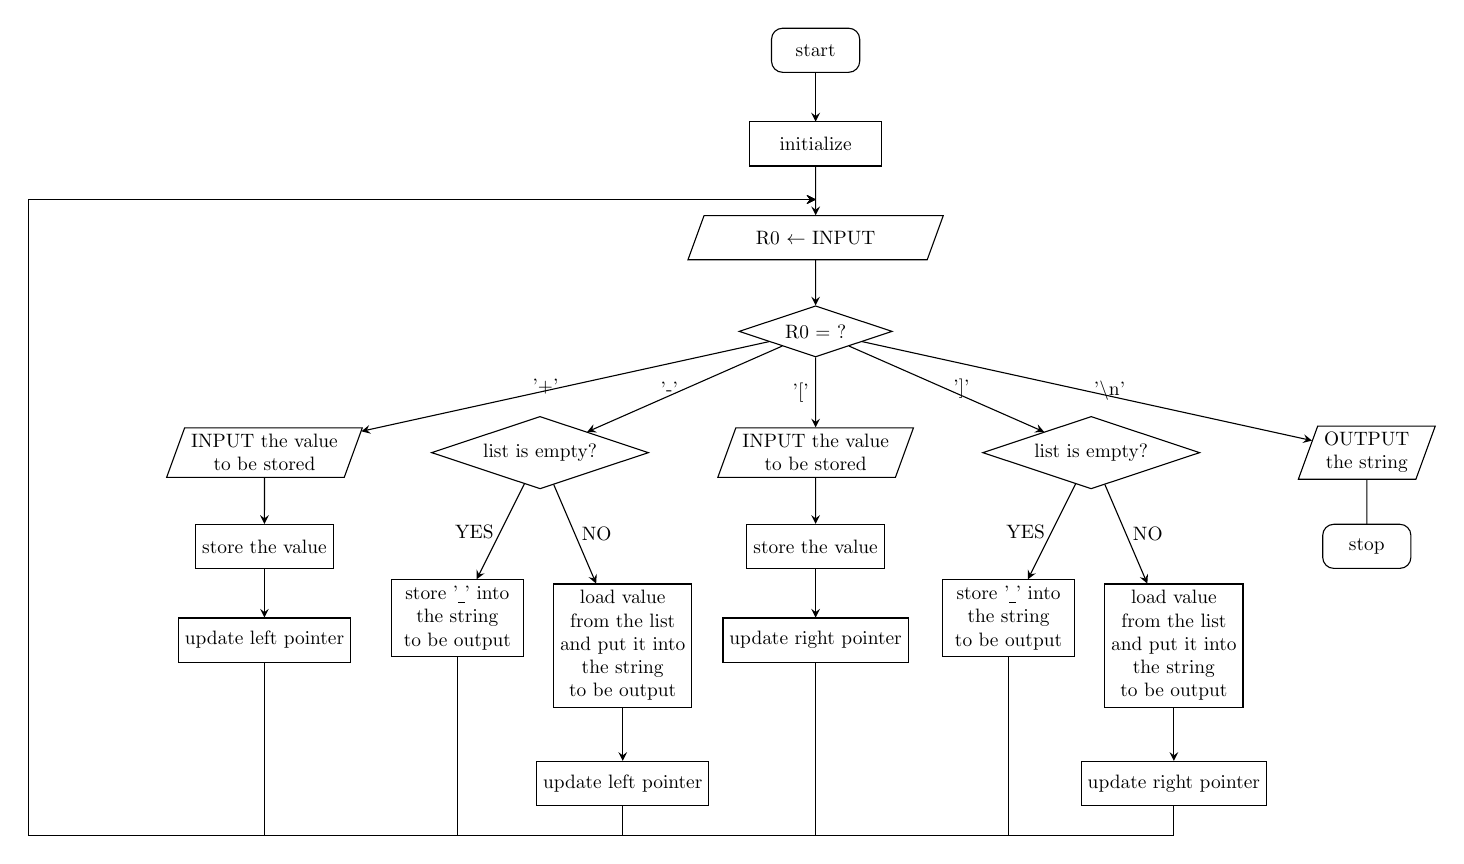
\begin{tikzpicture}[node distance=1.5cm, align=center]
  %定义流程图具体形状
  \node (start) [startstop] {start};
  \node (pro1) [process, below of=start, yshift= -0.2cm] {initialize};
  \node (in1) [io, below of = pro1, yshift = -0.2cm] {R0 $\leftarrow$ INPUT};
  \node (dec1) [decision, below of=in1, yshift= -0.2cm] {R0 = ?};

  % '+'
  \node (in2) [io, below of=dec1, yshift= -0.7cm, xshift = -10cm] {INPUT the value \\ to be stored};
  \node (pro2) [process, below of=in2, yshift= -0.2cm] {store the value};
  \node (pro3) [process, below of=pro2, yshift= -0.2cm] {update left pointer};

  % '-'
  \node (dec2) [decision, below of=dec1, yshift= -0.7cm, xshift = -5cm] {list is empty?};
  \node (pro4) [process, below of=dec2, yshift= -1.5cm, xshift = -1.5cm] {store '\underline{~}' into \\ the string \\ to be output};
  \node (pro5) [process, below of=dec2, yshift= -2cm, xshift = 1.5cm] {load value \\ from the list \\ and put it into \\ the string \\ to be output};
  \node (pro6) [process, below of=pro5, yshift= -1cm] {update left pointer};

  % '['
  \node (in3) [io, below of=dec1, yshift= -0.7cm] {INPUT the value \\ to be stored};
  \node (pro7) [process, below of=in3, yshift= -0.2cm] {store the value};
  \node (pro8) [process, below of=pro7, yshift= -0.2cm] {update right pointer};

  % ']'
  \node (dec3) [decision, below of=dec1, yshift= -0.7cm, xshift = 5cm] {list is empty?};
  \node (pro9) [process, below of=dec3, yshift= -1.5cm, xshift = -1.5cm] {store '\underline{~}' into \\ the string \\ to be output};
  \node (pro10) [process, below of=dec3, yshift= -2cm, xshift = 1.5cm] {load value \\ from the list \\ and put it into \\ the string \\ to be output};
  \node (pro11) [process, below of=pro10, yshift= -1cm] {update right pointer};

  % '\n'
  \node (out1) [io, below of=dec1, yshift= -0.7cm, xshift = 10cm] {OUTPUT \\ the string};
  \node (stop) [startstop, below of=out1, yshift= -0.2cm] {stop};

  %连接具体形状
  \draw [arrow](start) -- (pro1);
  \draw [arrow](pro1) -- (in1);
  \draw [arrow](in1) -- (dec1);

  \draw [arrow](dec1) -- node[anchor=east] {'+'} (in2);
  \draw [arrow](in2) -- (pro2);
  \draw [arrow](pro2) -- (pro3);
  \draw [arrow](pro3) -- ($(pro3.south) + (0, -2.2)$) -- ($(pro3.south) + (-3, -2.2)$) |- ($(in1.north) + (0, 0.2)$);

  \draw [arrow](dec1) -- node[anchor=east] {'-'} (dec2);
  \draw [arrow](dec2) -- node[anchor=east] {YES} (pro4);
  \draw [arrow](dec2) -- node[anchor=west] {NO} (pro5);
  \draw [arrow](pro5) -- (pro6);
  \draw [arrow](pro4) |- ($(pro3.south) + (0, -2.2)$) -- ($(pro3.south) + (-3, -2.2)$) |- ($(in1.north) + (0, 0.2)$);
  \draw [arrow](pro6) |- ($(pro3.south) + (0, -2.2)$) -- ($(pro3.south) + (-3, -2.2)$) |- ($(in1.north) + (0, 0.2)$);

  \draw [arrow](dec1) -- node[anchor=east] {'['} (in3);
  \draw [arrow](in3) -- (pro7);
  \draw [arrow](pro7) -- (pro8);
  \draw [arrow](pro8) |- ($(pro3.south) + (0, -2.2)$) -- ($(pro3.south) + (-3, -2.2)$) |- ($(in1.north) + (0, 0.2)$);

  \draw [arrow](dec1) -- node[anchor=west] {']'} (dec3);
  \draw [arrow](dec3) -- node[anchor=east] {YES} (pro9);
  \draw [arrow](dec3) -- node[anchor=west] {NO} (pro10);
  \draw [arrow](pro10) -- (pro11);
  \draw [arrow](pro9) |- ($(pro3.south) + (0, -2.2)$) -- ($(pro3.south) + (-3, -2.2)$) |- ($(in1.north) + (0, 0.2)$);
  \draw [arrow](pro11) |- ($(pro3.south) + (0, -2.2)$) -- ($(pro3.south) + (-3, -2.2)$) |- ($(in1.north) + (0, 0.2)$);

  \draw [arrow](dec1) -- node[anchor=west] {'$\backslash$n'} (out1);
  \draw (out1) -- (stop);
  \end{tikzpicture}
\caption{The flowchart of the program.}
\end{figure}

\newpage
\section{Source code}
\linespread{0.8}      %行距缩小
\begin{Verbatim}[frame = single, numbers = left, fontsize = \footnotesize]
.ORIG       x3000
            AND R0, R0, #0    ; initialize
            LD R5, START      ; R5 is the left of the queue
            ADD R5, R5, #1    ; R5 <-- x4001
            LD R6, START      ; R6 is the right of the queue
                              ; R6 <-- x4000
                              ; Both R5 and R6 points to the
                              ; next position of the top
            LEA R4, OUTSTR    ; R4 is the address of the output string
;
INPUT       GETC
            OUT
            LD R1, PLUS
            NOT R1, R1
            ADD R1, R1, #1
            ADD R1, R0, R1
            BRnp #2
            JSR LPUSH         ; input char is '+'
            BRnzp CONT
            LD R1, MINUS
            NOT R1, R1
            ADD R1, R1, #1
            ADD R1, R0, R1
            BRnp #2
            JSR LPOP          ; input char is '-'
            BRnzp CONT
            LD R1, LBRACKET
            NOT R1, R1
            ADD R1, R1, #1
            ADD R1, R0, R1
            BRnp #2
            JSR RPUSH         ; input char is '['
            BRnzp CONT
            LD R1, RBRACKET
            NOT R1, R1
            ADD R1, R1, #1
            ADD R1, R0, R1
            BRnp #2
            JSR RPOP          ; input char is ']'
            BRnzp CONT
            LD R1, LF
            NOT R1, R1
            ADD R1, R1, #1
            ADD R1, R0, R1
            BRnp #2
            JSR OUTPUT        ; input char is '\n'
            HALT
CONT        BRnzp INPUT       ; get next char
;
LPUSH       LD R0, LLIMIT
            NOT R0, R0
            ADD R0, R0, #1
            ADD R0, R0, R5
            BRz FULL
            GETC
            OUT
            STR R0, R5, #0    ; store the value
            ADD R5, R5, #1    ; and update the left pointer
            RET
;
LPOP        NOT R0, R6
            ADD R0, R0, #1
            ADD R0, R0, R5
            ADD R0, R0, #-1
            BRz EMPTY
            ADD R5, R5, #-1   ; update the left pointer
            LDR R0, R5, #0
            STR R0, R4, #0    ; store the value to the string to be output
            ADD R4, R4, #1
            RET
;
RPUSH       LD R0, RLIMIT
            NOT R0, R0
            ADD R0, R0, #1
            ADD R0, R0, R6
            BRz FULL
            GETC
            OUT
            STR R0, R6, #0    ; store the value
            ADD R6, R6, #-1   ; and update the left pointer
            RET
;
RPOP        NOT R0, R6
            ADD R0, R0, #1
            ADD R0, R0, R5
            ADD R0, R0, #-1
            BRz EMPTY
            ADD R6, R6, #1    ; update the right pointer
            LDR R0, R6, #0
            STR R0, R4, #0    ; store the value to the string to be output
            ADD R4, R4, #1
            RET
;
OUTPUT      LEA R0, OUTSTR
            PUTS
            RET
;
FULL        LEA R1, OVERFLOW
            AND R0, R0, #0
            ADD R0, R0, R1
            PUTS
            HALT
;
EMPTY       LD R0, UNDERLINE
            STR R0, R4, #0
            ADD R4, R4, #1
            RET
;
PLUS        .FILL x002B
MINUS       .FILL x002D
LBRACKET    .FILL x005B
RBRACKET    .FILL x005D
LF          .FILL x000A
UNDERLINE   .FILL x005F
START       .FILL x4000
RLIMIT      .FILL x4100
LLIMIT      .FILL x3E00
OVERFLOW    .STRINGZ "ERROR!OVERFLOW!"
OUTSTR      .BLKW x0200
.END
\end{Verbatim}
\linespread{0.9}      %行距恢复

\section{Questions TA asked you and your answer in check}
\noindent
如何更好地利用内存空间?即:当只从左侧插入右侧取出时,如何保证内存空间的合理利用?


\end{document}